\section{C++ Forbidden Forward Calls Exposed}
\label{C++ Bad Forward Indirect Calls}
\textbf{Polymorphism in C++.}
\label{Polymorphism in C++}
Polymorphism along inheritance and encapsulation
are the most used modern object-oriented concepts
in C++. 
Polymorphism in C++ allows to access different types of objects 
through a common base class. A pointer of the type of the base object
can be used to point to object(s) which are derived from the base class.
In C++ there are several types of polymorphism:
\textit{a)} compile-time (or static, usually is implemented with templates), 
\textit{b)} run-time (dynamic, is implemented with inheritance and virtual functions), 
\textit{c)} ad-hoc (e.g., if the range of actual types that can be used 
is finite and the combinations must be individually specified prior to use), and
\textit{d)} parametric (e.g., if code is written without mention of any 
specific type and thus can be used transparently with any number of new types it
is called parametric polymorphism). 
The first two are implemented through early 
and late binding, respectively.
In C++, overloading concepts fall under the category of \textit{c)} and Virtual functions;
templates or parametric classes fall under the category of pure polymorphism.
C++ provides polymorphism through: 
\textit{i)} virtual functions,
\textit{ii)} function name overloading, and 
\textit{iii)} operator overloading. 
In this paper, we will be concerned with dynamic 
polymorphism---based on virtual functions (10.3 and 11.5 in 
ISO/IEC N3690~\cite{iso:iecN3690})---because these can be exploited to 
call: 
\textit{x)} illegitimate vTable entries not/contained in the 
class hierarchy by varying or not the number of parameters and types,
\textit{y)} legitimate vTable entries not/contained in the
class hierarchy by varying or not the number of parameters and types,
\textit{z)} fake vTables entries not contained in the class hierarchy 
by varying or not the number of parameters and types.
By legitimate and illegitimate vTable entries we mean those 
vTable entries which for a single indirect call site lie in the 
vTable hierarchy. More precisely, a vTable entry is legitimate for 
a call site if from the call site to the vTable containing the entry there
is an inheritance path (see~\cite{haller:shrinkwrap}).
Virtual functions have several uses and issues associated, 
but for the scope of this paper we will look at the indirect 
call sites which are exploiter by calling illegitimate vTable entries (functions)
with varying number and type of parameters, \textit{x)}.
More precisely, 
\textit{1)} load-time enforcement: as calling each indirect call site (callee) requires 
a fix number of parameters which are passed each time the caller is calling, we
enforce a fine-grained CFI policy by statically determining the number and types of all function parameter
that belong to an indirect call site.
\textit{2)} run-time verification: as checking during run-time legitimate from
illegitimate indirect caller/callee pairs requires parameter type (along parameter number),
we check during run-rime before each indirect call-site if the caller matches to the callee 
based on the previously added checks.

\newsavebox{\firstlisting}
\begin{lrbox}{\firstlisting}
\begin{minipage}[c]{0.4\linewidth}
\begin{minted}[
% frame=lines,
framesep=2mm,
linenos,
frame=none,
firstnumber=1,
framesep = 1.0cm,
linenos,
numbersep=5pt,
%gobble=2,
%frame=lines,
framesep=2mm,
%fontsize=\tiny        
% baselinestretch=1.2,
% bgcolor=LightGray,
fontsize=\footnotesize,
]{C++}
class nsMultiplexInputStream final 
 :public nsIMultiplexInputStream //A0
 ,public nsISeekableStream //A1
 ,public nsIIPCSerializableInputStream //A2
 ,public nsICloneableInputStream{ //A3
nsTArray<nsCOMPtr<nsIInputStream>> mStreams;
NS_IMETHODIMP nsMultiplexInputStream::Close(){
  MutexAutoLock lock(mLock);
  mStatus = NS_BASE_STREAM_CLOSED;
  //set NS_OK flag
  nsresult rv = NS_OK;
  //get array length
  uint32_t len = mStreams.Length();
  //array-based main loop gadget
 for (uint32_t i = 0; i<len; ++i){
  //(1) hijacked indirect call
  nsresult rv2=mStreams[i]->Close();
  if (NS_FAILED(rv2)) {
      rv = rv2;
  }
 }
  return rv;
}
\end{minted}
\end{minipage}
\end{lrbox}

% \begin{figure}
%  \begin{minipage}[!t]{.40\linewidth}
%   \usebox{\firstlisting}
%  \end{minipage}%%
% \hfill
% \hspace{1.2cm}
% \begin{minipage}[!b]{.5\linewidth}
%    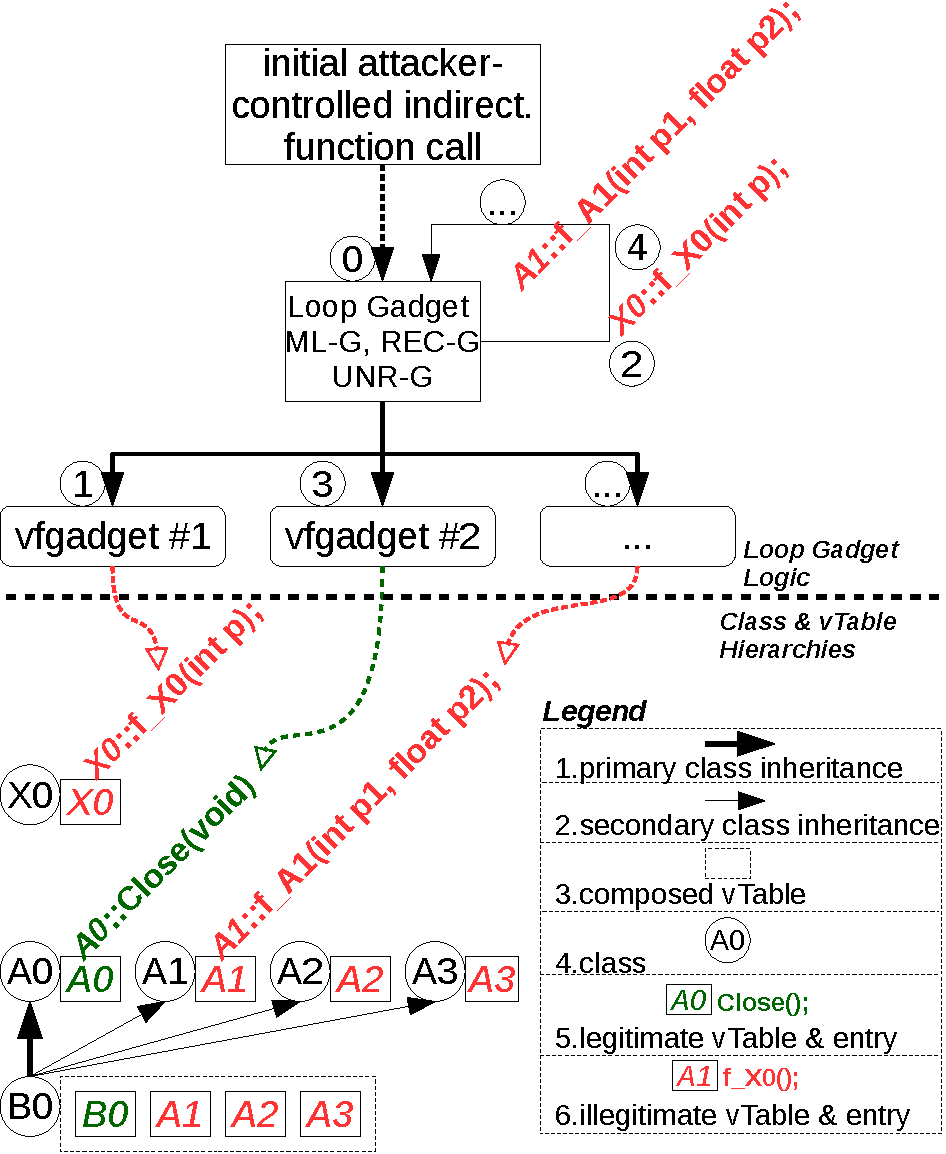
\includegraphics[width=1.3\textwidth]{figures/loop.pdf}
% \end{minipage}
% \caption{Code example used to illustrate how a COOP loop gadget works.}
% \label{Code example used to illustrate how a COOP loop gadget works}
% \end{figure}

%%%%%%%%%%%%%%%%%
\begin{figure}[!t]
   \centering
   \setlength{\unitlength}{0.1\textwidth}
   \begin{picture}(10,4)
     \put(2.85,0){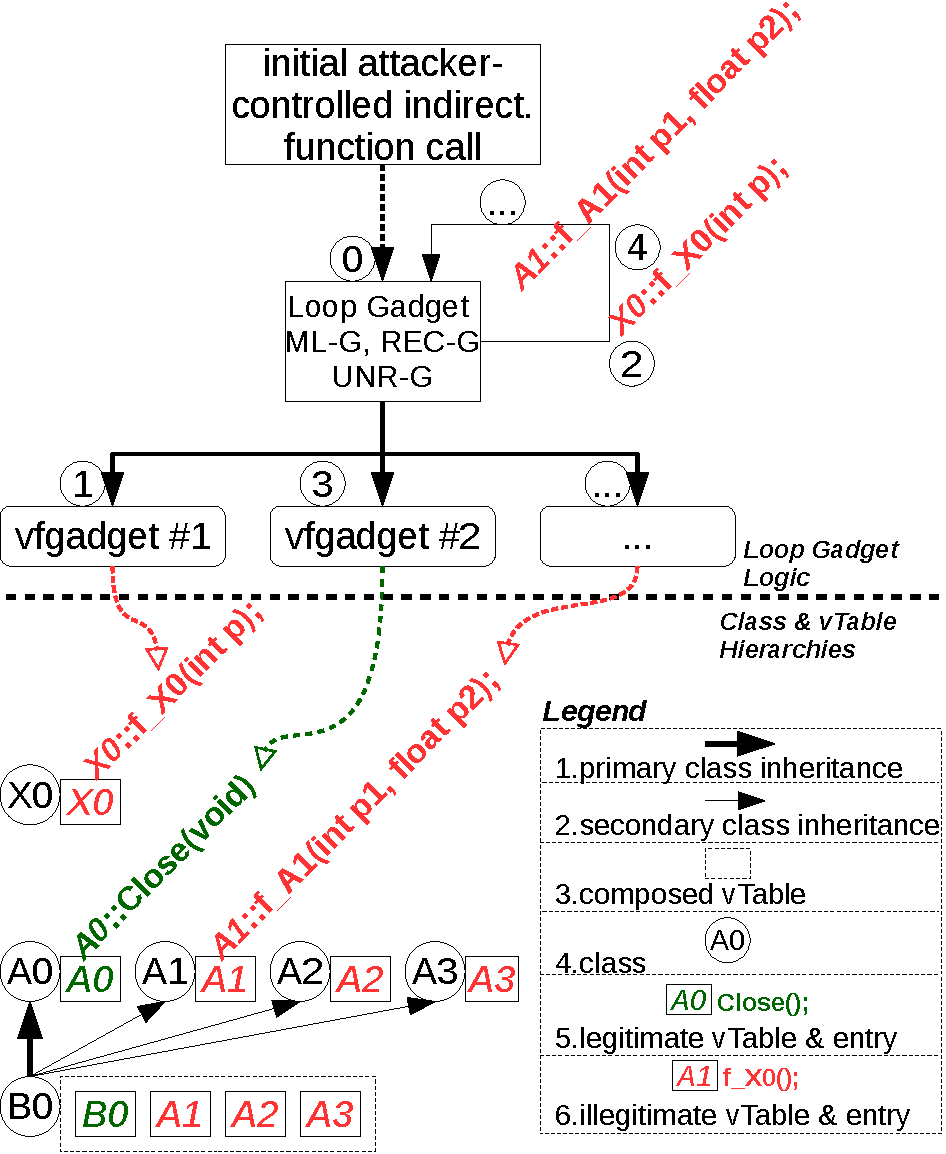
\includegraphics[width=.3\textwidth]{figures/loop.pdf}}
     \put(0,2){\usebox{\firstlisting}}
   \end{picture}
\caption{Code presenting how a COOP loop gadget works.}
\label{Code example used to illustrate how a COOP loop gadget works}
\end{figure}


Figure~\ref{Code example used to illustrate how a COOP loop gadget works}
depicts a C++ code example where it is illustrated how a COOP loop gadget 
(ML-G, REC-G, UNR-G, see~\cite{crane:readactor++}) works.
(1) can be exploited in several ways, see \textit{x), y) and z)}.
The indirect call site (line 17) can be exploited 
to call by passing a varying number of parameters and types
on each object contained in the array a different
vTable entry contained in the:
\textit{1)} class hierarchy (overall, whole program),
\textit{2)} class hierarchy (partial, only legitimate for this call site),
\textit{3)} vTable hierarchy (overall, whole program),
\textit{4)} vTable hierarchy (partial, only legitimate for this call site),
\textit{5)} vTable hierarchy and/or class hierarchy (partial, only legitimate for this call site), and
\textit{6)} vTable hierarchy and/or class hierarchy (overall, whole program).
There is no language semantics---such as cast checks---in C++ for vCall sites dispatch checking and as consequence
the loop gadget indicated in Figure~\ref{Code example used to illustrate how a COOP loop gadget works}
can basically call all around in the class and vTable hierarchy by not being constrained by any build in check during
run-time. The attacker corrupts an indirect function call, \circled{1}, 
next she invokes gadgets,  \circled{1}, \circled{3}, 
through the calls, \circled{2}, \circled{4}, contained in the loop. 
As it can be observed in in Figure~\ref{Code example used to illustrate how a COOP loop gadget works} she 
can invoke from the same call site legitimate functions residing in the vTable inheritance path
(this type of information is usually very hard to recuperate from executables)
for this particular call site, indicated with green color vTable entries. 
However, a real COOP attack invokes illegitimate
vTable entries residing in the whole initial program hierarchy (or the extended one)
with less or no relationship to the initial call site,
indicated with red color vTable entries.

\textbf{Checking Indirect Forward-Edge Calls in Practice.}
\label{C++ Indirect Calls in Practice}
As far as we know, there is only the IFCC/VTV~\cite{vtv:tice} tools (up to 8.7\% performance overhead) deployed in practice
which can be used to check legitimate from illegitimate indirect forward-edge calls during compile time.
vPointers are checked based on the class hierarchy. ShrinkWrap~\cite{haller:shrinkwrap} (as far as we know not deployed in practice)
is a tool which further reduces the legitimate vTbles ranges for a given indirect call site
through precise analysis of the program class hierarchy and vTable hierarchy. 
Evaluation results show similar performance overhead but more precision w.r.t. to legitimate vTables entries per call site.
We noticed by analyzing the previous research results that the overhead incurred by
these security checks can be very high due to the fact that for each call site many range checks 
have to be performed during run-time. Therefore, despite its security benefit these types of
checks can not be applied in our opinion to high performance applications.

As alternative, there are other highly promising tools (not deployed in practice) that can be used to mitigate 
some of the drawbacks of the previous tools. 
Bounov et al~\cite{bounov:interleaving} presented a tool ($\approx$ 1\% runtime overhead)
for indirect forward-edge call site checking based on vTable layout interleaving. The tool has better performance
than VTV and better precision w.r.t. allowed vTables per indirect call site. Its precision (selecting legitimate vTables for each call site)
compared to ShrinkWrap is lower since it does not consider vTable inheritance paths.
vTrust~\cite{zhang:vtrust} (average run-time overhead 2.2\%) enforces two layers of defense (virtual function type enforcement and vTable pointer sanitization)
against vTable corruption, injection and reuse.
TypeArmor~\cite{veen:typearmor} ($\le$ than 3 \% runtime overhead) enforces an CFI policy based on runtime checking of caller/caller pairs based
on function parameter count matching (coarse grained, parameter types and more than six parameters can be used as well).
Important to notice is that there are no C++ language semantics which can be used to enforce type and 
parameter count matching for indirect call/callee pairs, this could be addresses with specifically intended language constructs in future.

\textbf{Security Implications of Forbidden Indirect Calls.}
\label{Security Implications of Forbidden Forward Indirect Calls}
The C++ language standard (12.7~\cite{iso:iecN3690}) does not specify
what happens when calling different vTable entries from an indirect call site.
The standard says that we have have a virtual function related undefined behavior when:
``a virtual function call uses an explicit class member access and the object expression refers to the complete
object of x or one of that object’s base class subobjects but not x or one of its base class subobjects".
As undefined behavior is not a clearly defined concept we argue that in order to be able to deal
with undefined behavior or  unspecified behavior related to virtual function calls one needs to know
how these language dependent concepts are implemented inside the used compilers.

Forbidden forward-edge indirect calls are the result of a vPointer corruption.
A vPointer corruption is not a vulnerability but rather a capability which 
can be the result of a spatial or temporal memory corruption through: 
(1) bad-casting~\cite{byoungyoung:typecasting} of C++ objects, 
(2) buffer overflow in a buffer adjacent to a C++ object or a use-after-free condition~\cite{schuster:coop}.
A vPointer corruption can be exploited in several ways. A manipulated vPointer
can be exploited by pointing it in any existing or added program vTable entry 
or into a fake vTable which was added by an attacker. For example in case a vPointer
was corrupted than the attacker could highjack the control flow of the program 
and start a COOP attack~\cite{schuster:coop}.

vPointer corruptions are a real security threat which can be exploited if there 
is a memory corruption (e.g. buffer overflow) which is adjacent to
the C++ object or a use-after-free condition. As a consequence each corruption 
which can reach an object (e.g. bad object casts) is a potential exploit vector 
for a vPointer corruption. Interestingly to notice in this context is that through:
(1) memory layout analysis (through highly configurable compiler tool chains) of 
source code based locations which are highly prone to
memory corruptions such as declarations and uses of buffers, integers or pointer 
deallocations one can obtain the internal machine code layout representation.
(2) analysis of a code corruption which is adjacent (based on (1)) to a C++ object based on
application class hierarchy, the vTble hierarchy and each location in source code where an object
is declared and used (e.g., modern compiler tool chains can spill out this information for free), 
one can derive an analysis which can determine---up to a certain extent---if a memory corruption 
can influence (is adjacent) to a C++ object.

Finally, we notice that by building tools based on this two concepts (i.e., (1) and (2))
attackers (e.g., used to find new vulnerabilities) and for defenders which can 
harden the source code with checks only at the places which are most exposed 
to such vulnerabilities (i.e., we name this targeted security hardening).

\textbf{Real COOP Attack Example.}
\label{Running Example: CVE X}
The given example depicted in Figure~\ref{Class exploit}
is a proof of concept exploit extracted from~\cite{schuster:coop} and used in order to perform 
a COOP attack on the Firefox browser. A buffer overflow bug was used in order to call 
into existing vTable entries by using the a main loop gadget. 
The attack concludes with opening of an Unix shell. 
A real-world bug, CVE-2014-3176, was exploited by Crane et al.~\cite{crane:readactor++}
in order to perform another COOP attack on the Chromium browser. The details of the 
second attack are far to complex (i.e., involves not properly handled interaction of 
extensions, IPC, the sync API, and Google V8) and for this reason we briefly present the first 
documented COOP exploit on a Linux machine.

%%second pic
\begin{figure}[h]
    \centering
    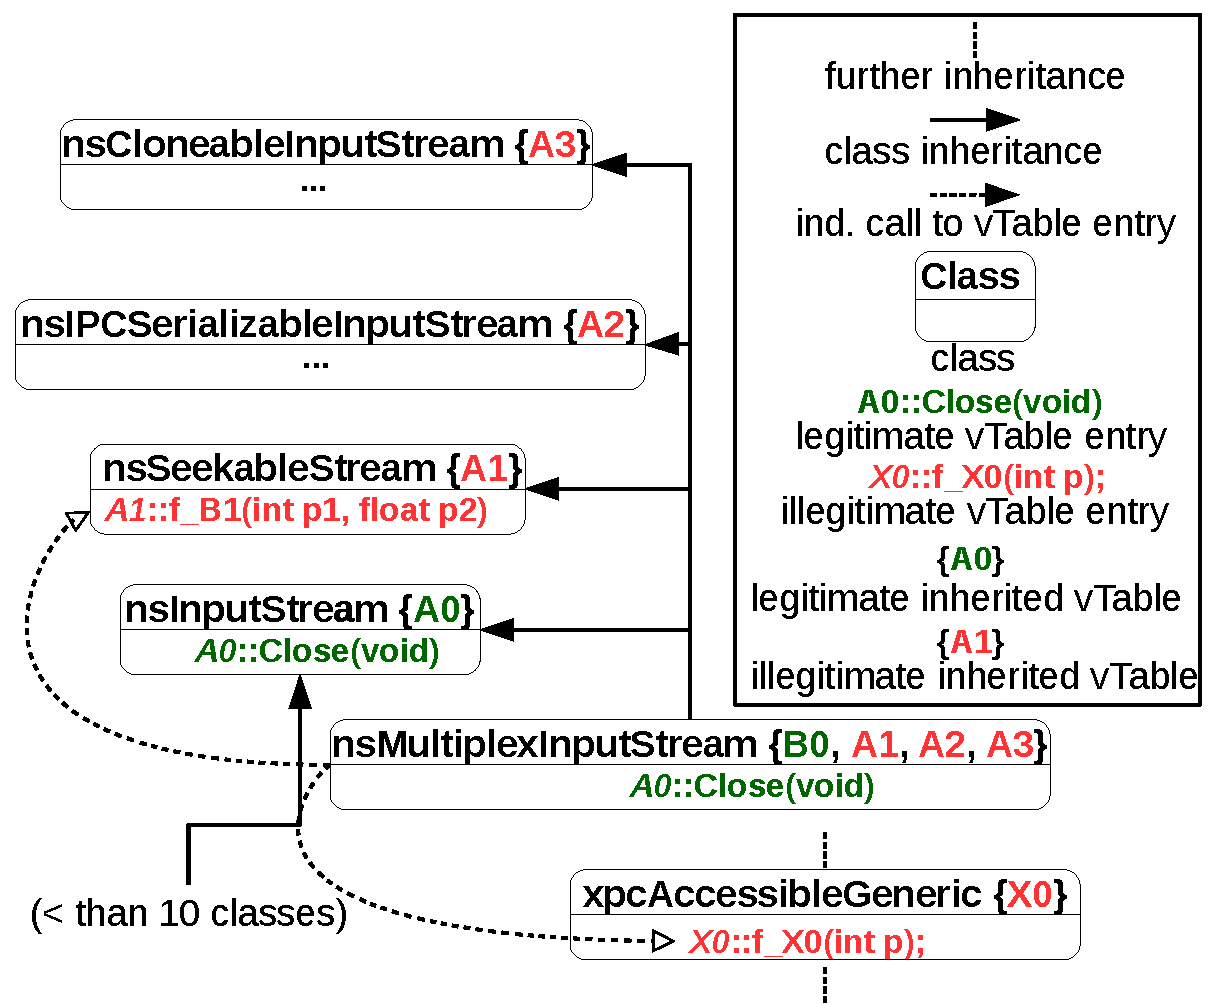
\includegraphics[width=0.47\textwidth]{figures/class_hierarchy.pdf}
\caption{Class inheritance hierarchy of the classes involved in the COOP attack against the Firefox browser. Red letters 
indicate forbidden vTble entries and green letters indicate allowed vTable entries for the given indirect call site
contained in the main loop gadget.}
\label{Class exploit}
\end{figure}

The C++ class \texttt{nsMultiplexInputStream} contains a main loop gadget inside the function 
\texttt{nsMultiplexInputStream::Close(void)} which is performing an indirect calls by dispatching
indirect calls on the objects contained in the array. 
The objects contained in the array during normal execution are of type \texttt{nsInputStream} and each
of the objects will call the \texttt{Close(void)} function in order to close each of the previously opened streams.
In order to perform the COOP attack the attacker crafts a C++ program containing a array buffer holding 
six fake objects. Fake objects can call inside (and outside) the initial class and vTable hierarchies
with no constraints.
During the attack a buffer is created in order to hold the fake objects.
The crafted buffer will be called in stead of the real code in order to call different functions
available in the program code. For example the attacker calls a function contained in the class
\texttt{xpcAccessibleGeneric} which is not in the class hierarchy or vTable hierarchy
of the initially intended type of objects used inside the array.
Moreover, the header file of this class (\texttt{xpcAccessibleGeneric}) is not included in the 
class \texttt{nsMultiplexInputStream}.
In total six fake objects are used to call into functions residing in not related class hierarchies with varying 
number of parameters and return types. The final goal of this attack is to prepare the program memory such 
that a Unix shell can be opened at the end of this attack.

This example illustrates why detecting vPointer corruptions is not trivial for real-world applications.
As depicted in Figure~\ref{Class exploit} the class \texttt{nsInputStream} has 11 classes which inherit directly
or indirectly from this class. The classes \texttt{nsSeekableStream}, \texttt{nsIPCSerializableInputStream}
and \texttt{nsClonea-\allowbreak bleInputStream} provide additional inherited vTables which represent illegitimate call targets
for the initial \texttt{nsInputStream} objects and legitimate call targets for the six fake objects which were added during the attack.
Furthermore, declaration and usage of the objects can be wide spread in the source code. This makes
detection of the object types (base class), range of vTables (longest vTable inheritance path for a particular call site)
and parameter types of the vTable entries (functions) in which it is allowed to call a 
trivial task for source code (current research work is mostly concerned with performance issues)
applications but a hard task in our opinion when one wants to apply similar security policies 
(e.g. which rely on parameter types of vTable entries) to executables.





